
%
\section{Introduction}\label{sec:intro}

%
%

Image recognition is central to computer vision, with dozens of new approaches being proposed every year, each optimized for particular aspects of the problem.
From coarse to fine, we may distinguish the recognition of
(a) classes, where one looks for a certain type of object regardless of intra-class variations,
(b) instances, where one looks for a particular object despite changes in the viewing conditions,  and
(c) copies, where one looks for a copy of a specific image despite edits.
While these problems are in many ways similar, the standard practice is to use specialized, and thus incompatible, image representations for each case.

Specialized representations may be accurate, but constitute a significant bottleneck in some applications.
Consider for example image retrieval, where the goal is to match a query image to a large database of other images.
Very often one would like to search the same database with multiple granularities, by matching the query by class, instance, or copy.
The performance of an image retrieval system depends primarily on the \emph{image embeddings} it uses. 
These strike a trade-off between database size, matching and indexing speed, and retrieval accuracy.
Adopting multiple embeddings, narrowly optimized for each type of query, means multiplying the resource usage.

\begin{figure}
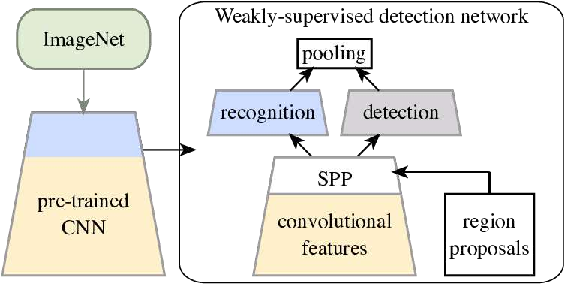
\includegraphics[width=1.\linewidth]{figs/splash}
\vspace{-10pt}
\caption{Our goal is to extract an image descriptor incorporating different levels of granularity, so that we can solve, in particular, classification and particular object recognition tasks: The descriptor is either fed to a linear classifier, or directly compared with cosine similarity. 
%
\label{fig:splash}} 
\vspace{-10pt}
\end{figure}


In this paper we present a new  representation, MultiGrain, that can achieve the three tasks together, regardless of differences in their semantic granularity, see \cref{fig:splash}.
We learn MultiGrain by jointly training an image embedding for multiple tasks.
The resulting representation is compact and outperforms narrowly-trained embeddings.

Instance retrieval has a wide range of industrial applications, including detection of copyrighted images and exemplar-based recognition of unseen objects.
In settings where billion of images have to be treated, %
it is of interest to obtain image embeddings suitable for more than one recognition task.
For instance, an image storage platform is likely to perform some classification of the input images, aside from detecting copies or instances of the same object.
An embedding relevant to all these tasks advantageously reduces both the computing time per image and storage space.

In this perspective, convolutional neural networks (CNNs) trained only for classification already go a long way towards universal features extractors. %
%
%
The fact that we can learn image embeddings that are simultaneously good for classification and instance retrieval is surprising but not contradictory.
In fact, there is a logical dependence between the tasks: images that contain the same instance also contain, by definition, the same class; and copied images contain the same instance.
%
This is in contrast to multi-task settings where tasks are in competition and are thus difficult to combine.
Instead, both class, instance, and copy congruency lead to embeddings that should be close in feature space.
Still, the degree of similarity is different in the different cases, with classification requiring more invariance to appearance variations and copy detection sensitivity to small image details.

%
%
%
%
%
%

In order to learn an image representation that satisfies the different trade-offs, we start from an existing image classification network.
We use a generalized mean layer %
that converts a spatial activation map to a fixed-size vector.
%
%
Most importantly, we show that it is an effective way to learn an architecture that can adapt to different resolutions \emph{at test time}, and offer higher accuracies. This circumvents the massive engineering and computational effort needed to learn networks for larger input resolutions~\cite{He2016IdentityMI}

The joint training of classification and instance recognition objectives is based on cross-entropy and contrastive losses, respectively.
Remarkably, instance recognition is learned for free, \emph{without using labels specific to instance recognition or image retrieval}: we simply use the identity of the images as labels, and data augmentation as a way to generate different versions of each image. %
%

In summary, our main contributions are as follows: 
\begin{itemize}
    \item We introduce the MultiGrain architecture, which outputs an image embedding incorporating different levels of granularity. Our dual classification+instance objective improves the classification accuracy on its own. %
    \item We show that part of this gain is due to the batching strategy, where each batch contains repeated instances of its images with different data augmentations for the purpose of the retrieval loss; %
    %
    \item We incorporate a pooling layer inspired by image retrieval. It provides a significant boost in classification accuracy when provided with high-resolution images.
\end{itemize}
Overall, our architecture offers competing performance both for classification and image retrieval. Noticeably, we report a significant boost in accuracy on Imagenet with a ResNet-50 network over the state of the art. 


%

The paper is organized as follows. \Cref{sec:related} introduces related works. \Cref{sec:arch} introduces our architecture, the training procedure and explains how we adapt the resolution at test time. \Cref{sec:experiments} reports the main experiments. %
